\chapter{Analisi dei Requisiti}
\label{cap:analisi-requisiti}

Il seguente capitolo di Analisi dei Requisiti rappresenta una dettagliata e approfondita esplorazione delle necessità e delle aspettative che guidano la creazione e lo sviluppo del progetto in questione. Questa analisi è stata condotta al fine di definire chiaramente gli obiettivi e le funzionalità del prodotto, fornendo una base solida per la progettazione e l'implementazione del software.\\

\section{Descrizione generale}
Ogni caso d'uso è stato schematizzato secondo i seguenti punti:
\begin{itemize}
\item \textbf{attore coinvolto:} in cui si specifica l'attore;
\item \textbf{descrizione:} offre una spiegazione più dettagliata del caso d'uso; 
\item \textbf{precondizioni:} rappresenta la condizione che deve essere soddisfatta e verificata affinchè il caso d'uso possa essere eseguito con successo;
\item \textbf{postcondizioni:} rappresenta lo stato dell'attore in seguito all'esecuzione con successo del caso d'uso;
\item \textbf{estensioni:} in cui si specificano le eventuali estensioni collegate;
\item \textbf{inclusioni:} in cui si specificano le eventuali inclusioni.
\end{itemize}
Vengono inserite anche delle immagini dell'UML\textsubscript{g} per fornire una spiegazione visiva che può aiutare maggiormente la comprensione.

\section{Semplificazioni adottate nei casi d'uso}
All'interno dei casi d'uso è possibile leggere l'abbreviazione "vis." . Il seguente termine è utilizzato per abbreviare la parola "Visualizzazione".\\
Per agevolare la lettura delle immagini dei casi d'uso non è stato inserito il collegamento tra gli scenari principali e il database. È dato per scontato quindi, che ogni informazione venga recuperata dal database.\\

\section{Attori}
\begin{figure}[H] 
    \centering 
    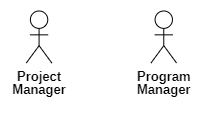
\includegraphics[width=0.3\columnwidth]{attori} 
    \caption{Attori}
\end{figure}
Gli attori che possiamo trovare all'interno dei casi d'uso rappresentano due risorse aziendali:
\subsubsection*{Project Manager}
Conosciuto come il "Responsabile di Progetto", si occupa dell'avvio, pianificazione ,esecuzione e controllo di un singolo progetto, seguendo tecniche di project management.\\
Le sue principali responsabilità sono:
\begin{itemize}
\item assicurarsi che i progetti siano allineati con gli obiettivi aziendali;
\item coordinare le risorse umane, assicurandosi che vengano utilizzate in modo efficiente;
\item stabilisce milestone, scadenze e obiettivi, monitorando lo stato di avanzamento dei progetti;
\item comunica con stakeholder, team di progetto e altre parti interessate.
\end{itemize}
\subsubsection*{Program Manager}
È un ruolo di gestione all'interno di un'organizzazione, ed è responsabile della pianificazione complessiva e del controllo di più progetti che compongono il suo programma. Collabora strettamente col Project Manager ed i loro compiti spesso si sovrappongono ma differiscono di portata, in quanto il Program Manager supervisiona gruppi di progetti gestiti singolarmente dai Project Manager.

\section{Casi d'uso}
\subsection{Primo caso}


\section{Tracciamento dei requisiti}


 

